\subsection{Atomistic Spin Hamiltonian}

\paragraph{Equation.}
Following the ASTRO exchange-sign convention, a classical spin Hamiltonian
containing exchange, uniaxial anisotropy, Dzyaloshinskii--Moriya interaction,
and Zeeman energy is
\begin{align}
    \mathcal{H}
    ={} & +\frac{1}{2}\sum_{i\ne j} J_{ij}\,\svec_i\cdot\svec_j
    -\sum_i K_i\bigl(\svec_i\cdot\unitvect{e}_i\bigr)^2
    \notag                                                      \\
        & -\frac{1}{2}\sum_{i\ne j}
    \vect{D}_{ij}\cdot(\svec_i\times\svec_j)
    -\sum_i \vect{\mu}_i\cdot\Bext.
    \label{eq:atomistic-hamiltonian}
\end{align}

\paragraph{Definitions.}
$J_{ij}$ is the exchange-link energy in the ASTRO sign convention: $J_{ij}<0$
favors parallel alignment, whereas $J_{ij}>0$ favors antiparallel alignment.
$K_i$ is the uniaxial anisotropy energy, $\unitvect{e}_i$ is the easy-axis
direction, $\vect{D}_{ij}$ is the Dzyaloshinskii--Moriya vector, and
$\vect{\mu}_i$ is the magnetic moment at site $i$.

\paragraph{Assumptions.}
Each $\svec_i$ is a classical unit vector.  The pair coefficients satisfy
$J_{ji}=J_{ij}$ and $\vect{D}_{ji}=-\vect{D}_{ij}$.  The factors of $1/2$
assume that the pair sums include both ordered pairs $(i,j)$ and $(j,i)$.
If each physical bond is instead included only once, for example in a
unique-bond sum $\sum_{\langle i,j\rangle}$, both factors of $1/2$ must be
omitted.  These are equivalent pair-counting conventions and must not be mixed.

Figure~\ref{fig:atomistic-bond-interactions} collects the geometric quantities
attached to one bond and distinguishes a physical bond from its two ordered
appearances in the Hamiltonian sum.

\begin{figure}[htbp]
    \centering
    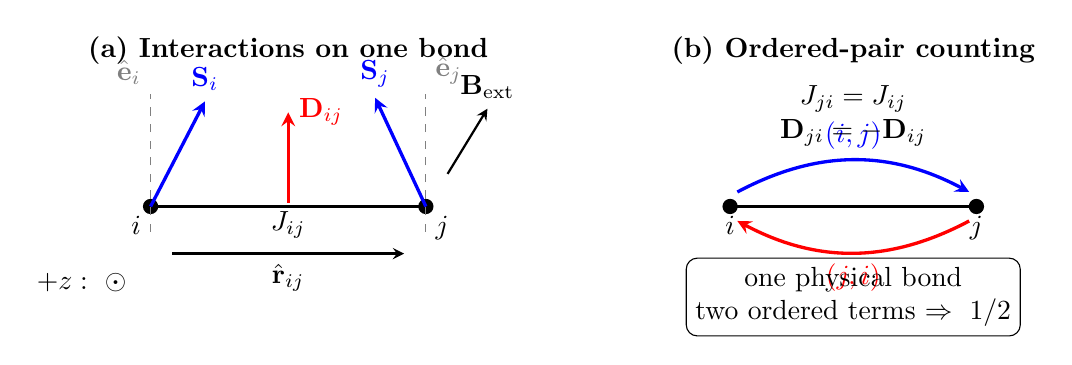
\begin{tikzpicture}[>=stealth,scale=0.92]
        \begin{scope}
            \node[font=\bfseries] at (2.45,2.15)
                {(a) Interactions on one bond};

            \draw[very thick] (0.55,0) -- (4.35,0);
            \fill (0.55,0) circle (3pt) node[below left] {$i$};
            \fill (4.35,0) circle (3pt) node[below right] {$j$};
            \node at (2.45,-0.25) {$J_{ij}$};

            \draw[->,very thick,blue] (0.55,0) -- (1.3,1.45)
                node[above] {$\mathbf{S}_i$};
            \draw[->,very thick,blue] (4.35,0) -- (3.65,1.5)
                node[above] {$\mathbf{S}_j$};
            \draw[dashed,gray] (0.55,-0.35) -- (0.55,1.55)
                node[above left] {$\hat{\mathbf e}_i$};
            \draw[dashed,gray] (4.35,-0.35) -- (4.35,1.55)
                node[above right] {$\hat{\mathbf e}_j$};

            \draw[->,thick] (0.85,-0.65) -- (4.05,-0.65)
                node[midway,below] {$\hat{\mathbf r}_{ij}$};
            \draw[->,very thick,red] (2.45,0.05) -- (2.45,1.3)
                node[right] {$\mathbf D_{ij}$};
            \draw[->,thick] (4.65,0.45) -- (5.2,1.35)
                node[above] {$\mathbf B_{\mathrm{ext}}$};
            \node[anchor=east] at (0.35,-1.05) {$+z:\ \odot$};
        \end{scope}

        \begin{scope}[xshift=8cm]
            \node[font=\bfseries] at (2.25,2.15)
                {(b) Ordered-pair counting};
            \draw[very thick] (0.55,0) -- (3.95,0);
            \fill (0.55,0) circle (3pt) node[below] {$i$};
            \fill (3.95,0) circle (3pt) node[below] {$j$};

            \draw[->,very thick,blue] (0.65,0.2)
                to[bend left=28] node[above] {$(i,j)$} (3.85,0.2);
            \draw[->,very thick,red] (3.85,-0.2)
                to[bend left=28] node[below] {$(j,i)$} (0.65,-0.2);
            \node[align=center] at (2.25,1.25)
                {$J_{ji}=J_{ij}$\\$\mathbf D_{ji}=-\mathbf D_{ij}$};
            \node[draw,rounded corners,align=center] at (2.25,-1.25)
                {one physical bond\\two ordered terms $\Rightarrow\ 1/2$};
        \end{scope}
    \end{tikzpicture}
    \caption{Original schematic of the bond quantities in
    Eq.~\eqref{eq:atomistic-hamiltonian}.  Panel (a) shows two spins, their local
    easy axes, the exchange link, the directed bond, the DMI vector, and the
    external field.  The displayed DMI orientation illustrates the ASTRO
    convention $\mathbf D_{ij}=D(\hat{\mathbf z}\times
    \hat{\mathbf r}_{ij})$.  Panel (b) shows why an ordered-pair sum contains
    both $(i,j)$ and $(j,i)$ and therefore carries a factor $1/2$
    ~\cite{astro-code}.}
    \label{fig:atomistic-bond-interactions}
\end{figure}

\paragraph{Pair counting and effective field.}
Let $\mu_i=\abs{\vect{\mu}_i}$ and define the effective flux density by
\begin{equation}
    \vect{B}_{\mathrm{eff},i}
    =-\frac{1}{\mu_i}\frac{\partial\mathcal{H}}{\partial\svec_i}.
    \label{eq:atomistic-effective-field}
\end{equation}
For the ordered-pair Hamiltonian above, the exchange and DMI contributions are
\begin{equation}
    \vect{B}_{\mathrm{ex},i}
    =-\frac{1}{\mu_i}\sum_{j\ne i}J_{ij}\svec_j,
    \qquad
    \vect{B}_{\mathrm{DMI},i}
    =\frac{1}{\mu_i}\sum_{j\ne i}\svec_j\times\vect{D}_{ij}.
    \label{eq:atomistic-pair-fields}
\end{equation}
The two ordered occurrences of each bond give identical derivatives, which
cancel the Hamiltonian factors of $1/2$.  Consequently, no extra factor of
$1/2$ belongs in either effective-field expression.

\paragraph{Units.}
All terms in $\mathcal{H}$ have units of energy.  Here the external flux density
$\Bext$ is measured in tesla, so no additional factor of $\mu_0$ appears in the
Zeeman term.

\paragraph{Source.}
For the extended classical spin Hamiltonian and Hamiltonian-derivative field
convention, see Evans et al.~\cite{evans2014atomistic}.

\paragraph{Implementation notes.}
The ASTRO implementation evaluates the field,
$\vect{B}_{\mathrm{eff},i}=-(1/\mu_i)\,\partial\mathcal{H}/\partial\svec_i$,
rather than the total energy and includes both forward and backward nearest
neighbors.  The $J_{ij}$ used above is therefore the coefficient stored in
ASTRO's exchange-link arrays: its exchange field is
$-(1/\mu_i)\sum_jJ_{ij}\svec_j$~\cite{astro-code}.  No factor of $1/2$ should
appear in the exchange or DMI field formulas because differentiation produces
two identical bond contributions, cancelling the Hamiltonian factor.  ASTRO's
DMI component expressions correspond to
$\vect{D}_{ij}=D(\unitvect{z}\times\unitvect{r}_{ij})$ and the antisymmetry
$\vect{D}_{ji}=-\vect{D}_{ij}$ used above.
